\documentclass[aps,reprint]{revtex4-1}
% Engine-specific settings
% Detect pdftex/xetex/luatex, and load appropriate font packages.
% This is inspired by the approach in the iftex package.
% pdftex:
\ifx\pdfmatch\undefined
\else
    \usepackage[T1]{fontenc}
    \usepackage[utf8]{inputenc}
\fi
% xetex:
\ifx\XeTeXinterchartoks\undefined
\else
    \usepackage{fontspec}
    \defaultfontfeatures{Ligatures=TeX}
\fi
% luatex:
\ifx\directlua\undefined
\else
    \usepackage{fontspec}
\fi
% End engine-specific settings
\usepackage[english]{babel}
\usepackage{csquotes}
% \usepackage[backend=biber, sortcites]{biblatex}
\usepackage{url}
\usepackage{textcomp}
\usepackage[usenames,dvipsnames,svgnames, table]{xcolor}
\usepackage[font={scriptsize}]{caption}
\usepackage{amsmath} \usepackage{amsthm} \usepackage{amsfonts}
\usepackage{amssymb}
\usepackage{enumerate}
\usepackage{tikz}
\usetikzlibrary{backgrounds}
\usepackage{float}
\usepackage[procnames]{listings}
\usepackage{pstool} \usepackage{pgfplots}
\usepackage{wrapfig} \usepackage{graphicx} \usepackage{epstopdf}
\usepackage{afterpage}
\usepackage{physics}
\usepackage{multirow}
\usepackage{gensymb}
\usepackage{algorithm}
\usepackage{microtype}
\usepackage[noend]{algpseudocode}
\usepackage{xcolor,colortbl}
\usepackage{microtype}
\usepackage{geometry}
\usepackage{hyperref}
\usepackage{graphicx}
\usepackage{caption}
\usepackage{subcaption}
\usepackage{lipsum}
% \usepackage{pythontex}
% \usepackage{authblk}
\usepackage{nth}
\usepackage{siunitx}
% \usepackage[toc,page]{appendix}
\floatstyle{plaintop}
\restylefloat{table}

% Custom commands
\newcommand{\unit}[1]{\:\mathrm{#1}}
\newcommand{\noref}[1]{\hyperref[#1]{\ref*{#1}}}
\newcommand{\nonref}[1]{\hyperref[]{\ref*{#1}}}
\newcommand\blankpage{%
  \null
  \thispagestyle{empty}%
  \addtocounter{page}{-1}%
  \newpage}
\newcommand{\mean}[1]{\langle #1 \rangle}

% Default fixed font does not support bold face
\DeclareFixedFont{\ttb}{T1}{txtt}{bx}{n}{7} % for bold
\DeclareFixedFont{\ttm}{T1}{txtt}{m}{n}{7}  % for normal

\newcommand\numberthis{\addtocounter{equation}{1}\tag{\theequation}}
\DeclareCaptionFont{white}{\color{white}}
\DeclareCaptionFormat{listing}{\colorbox{gray}{\parbox{\columnwidth}{#1#2#3}}}
\pgfplotsset{compat=1.14} %TODO: Setting this removed several error messages, should it be here!?


% Biber for references
% \bibliographystyle{aipauth4-1}

\begin{document}
\sisetup{detect-all}
\title{Ising model for studies of phase transitions in magnetic systems - A computational approach}
\author{Frederik J. Mellbye}
\affiliation{University of Oslo, Oslo, Norway \\ Source code available at: \url{https://github.com/Caronthir/FYS3150/tree/master/Project4}}
\date{\today}

\begin{abstract}\noindent
Once again the abstract abstractifies the abstractness of the abstract mathematical
equations than govern the universe.

\bigskip
\noindent \textbf{Disclaimer}:
\newline
For this project I collaborated with Erlend Lima with regards to the
analytic solutions presented, the code and therefore results and figures.
The text in this paper is written entirely by F. Mellbye, however there may be
several similarities with the Lima's paper, because the ideas and solutions
were discussed and developed together.
\end{abstract}
\maketitle
\tableofcontents
\makeatletter
\let\toc@pre\relax
\let\toc@post\relax
\makeatother

\newpage

\section{Introduction} \label{sec:introduction}
The Ising model is a widely used model, because of a wide range of applications,
for instance in studies of phase transitions to simulations in statistics.
\section{Theory} \label{sec:theory}
\subsection{The Ising model}
A square lattice of $N \times N$ binary magnetic dipoles (quantified atomic spins)
make up the Ising model. The dipoles can only have spins $s_i$ up ($1$) and down ($-1$).
In the Ising model the temperature $T$ is held constant.

The energy is given by
\begin{align}\label{eq:energy}
  E = -J \sum_{\langle kl \rangle}^{N} s_k s_l
\end{align}
where for each lattice location the sum is taken over the neighbors only. $J$ is
a constant that determines the strength of the interaction between the nodes
(The complexity of the quantum mechanics in such a system is baked into
this constant). It is assumed that there is a ferromagnetic ordering so that $J > 0$.
There is also an additional term if an external magnetic field is applied, but
in this paper this is set to $0$.

The magnetization is simply given as the sum of the spins:
\begin{align}\label{eq:magmom}
  \mathcal{M} = \sum_i s_i
\end{align}

The thermodynamical quantities that are computed in this paper can be constructed
from the above expressions. The heat capacity under constant volume $C_V$ is given
by
\begin{align}\label{eq:Cv}
  C_V = \frac{\mean{E^2} - \mean{E}^2}{kT^2}
\end{align}
and the magnetic suceptibility is similarly given by
\begin{align}\label{eq:sus}
  \chi = \frac{\mean{\mathcal{M}^2} - \mean{\mathcal{M}}^2}{kT}
\end{align}
For a more extensive explaination and derivation of the above expressions see
\cite{mortenjensen}. Another equation which is also presented in the lecture notes
is a way to compute the expectation value of the energy $\mean{E}$:
\begin{align}\label{eq:meanE}
  \mean{E} = - \pdv{\ln{Z}}{\beta}
\end{align}

\subsection{Boundary conditions}
There are several ways to model the boundaries, which have different advantages
and disadvantages. Perhaps the easiest solution is for the boundary spins to have
no outside neighbors. Usually real materials have an enormous amount of spins,
and the effect of the boundaries is negligible. In the Ising model an infinite
number of spins is not possible, and for small lattice sizes an appropriate
method needs to be used. For the intents and purposes of this paper, an ideal
method is to have so-called periodic boundaries. This involves treating the
spins on the oppsite side of the lattice as the neighbors of the boundary spins.
This is a much better approximation to an infinitely large lattice, because
each spin has access to four neighbors.

\subsection{Metropolis algorithm}
Monte-Carlo simulations are used to model the time development of the system.
With some initial configuration, an algorithm that over time modifies the system
to an equilibrium state needs to be employed. A method which has been shown to
do this is the famous Metropolis algorithm. See chapter .. in CITE for a detailed explaination
of the algorithm, the main steps are as follows:
\begin{enumerate}
  \item Select randomly $N^2$ spins in the lattice.
  \item Calculate the system change in energy $\Delta E$ if a randomly selected spin was to
  be flipped.
  \item Draw a random number from the uniform distribution, and compare
  \begin{align*}
    U(0,1) \leq e^{-\beta \Delta E}.
  \end{align*}
  If this is true, the spin is flipped. If this evaluates as false, do not flip
  the spin. If $\Delta E < 0$ the spin is flipped regardless, to model that physical
  systems usually tend to lower energy configurations.
\end{enumerate}
When this is repeated multiple times the system will converge to the equilibrium
state. In this model, the system development with Monte-Carlo cycles can therefore be
considered the system development with time.
\subsection{Phase transitions in the Ising model}
One of the properties of the Ising model is that phase transitions can be
observed. The transition occurs at a critical temperature $T = T_C$, where
the spins fluctuate at a maximum rate. The rapid fluctuations result in high
variances in energy and magnetic moment, i.e. a maximum for the heat capacity
and susceptibility. According to \cite{project4} these quantities can be
modelled as
\begin{align*}
  \mean{M(T)} &\sim (T - T_C)^\beta \\
  C_V(T) &\sim |T_C - T|^\gamma \\
  \chi (T) &\sim |T_C - T|^{-\alpha}
\end{align*}
where $\alpha = 0$, $\beta = 1/8$ and $\gamma = 7/4$ are critical exponents.
\subsection{Analytic solution in the 2 x 2 lattice case}
For the simple case of a $2 \times 2$ periodic boundary lattice analytic
expressions can be computed, which will be used to check that the numerical
implementation produces acceptable results. The four spins are enumerated as in
figure ~\ref{fig:22lattice}.
\begin{figure}[H]
  \centering
  \begin{tikzpicture}[thick]
    \draw[->] (0,0) -- (0,.3)  node [label=left:{$s_1$}] {};
    \draw[->] (1,0) -- (1,.3)  node [label=right:{$s_2$}] {};
    \draw[->] (0,1) -- (0,1.3) node [label=left:{$s_3$}] {};
    \draw[->] (1,1) -- (1,1.3) node [label=right:{$s_4$}] {};
    \draw[dotted] (-.75,-.4) rectangle (1.75,1.9);
  \end{tikzpicture}
  \caption{$2 \times 2$ enumerated lattice with all spins pointing up.}
  \label{fig:22lattice}
\end{figure}
A short walkthrough and the relevant equations are presented here, the equations
and derivations are entirely based on \cite{mortenjensen}. In a $2 \times 2$
lattice, there are $2^4 = 16$ possible microstates (unique configurations). Each
microstate is associated with thermodynamical quantities, such as energy and
magnetization, which determines the partition function. From this it is possible
to derive multiple statistical properties of the system.

Energies and magnetizations for the different possible configurations were calculated
using the method presented in the lecture notes by Hjort-Jensen.
The results of the calculations are shown in table ~\ref{tab:2x2values}.

\begin{table}[H]
  \caption{Possible states and associated energies, magnetizations and degeneracies.
  The same table is also found in \cite{mortenjensen}}
  \label{tab:2x2values}
  \begin{ruledtabular}
    \begin{tabular}{cccc}
      Spins up & Energy [$J$] & Magnetization & Multiplicity \\
      4        & -8           & 4             & 1            \\
      3        & 0            & 2             & 4            \\
      2        & 0            & 0             & 4            \\
      2        & 8            & 0             & 2            \\
      1        & 0            & -2            & 4            \\
      0        & -8           & 4             & 1
    \end{tabular}
  \end{ruledtabular}
\end{table}
With the entries in the above table it is possible to calculate the partition
function, which is given by
\begin{align} \label{eq:partitionfunc}
  Z = \sum_i e^{\beta E_i}
\end{align}
where $\beta = 1/kT$. By simply summing over all the microstates with equation ~\ref{eq:partitionfunc}
one finds
\begin{align*}
  Z = 2 e^{8\beta J} + 2 e^{- 8\beta J} + 12 = 4 \cosh{(8\beta J)} + 12
\end{align*}
When the partition function is known, the statistical thermodynamical quantities
of interest can be computed. To save space the alebra is pushed to the appendix,
and the relevant expressions are listed here:

The mean energy (energy expectation value) is given by
\begin{align*}
  \mean{E} = -\frac{8 J \sinh{(8\beta J)}}{\cosh{(8\beta J)} + 3}
\end{align*}
and the mean of the square of the energy is given by
\begin{align*}
  \mean{E^2} = \frac{256 J^2 \cosh{(8\beta J)}}{4\cosh{8\beta J} + 12}.
\end{align*}
The energy expressions can be used to compute the heat capacity $C_V$, which
is given by
\begin{align*}
  C_V = \frac{1}{kT} \left( \mean{E^2} - \mean{E}^2 \right)
\end{align*}

Similarly, the magnetization properties are given by
\begin{align*}
  \mean{M} &= 0 \\
  \mean{M^2} &= \frac{8e^{8 J \beta} + 8}{\cosh{8\beta J} + 3}
\end{align*}
which can be used to find the susceptibility using equation ~\ref{eq:sus}.

\section{Method} \label{sec:method}
All of the numerical calculations were done in C++, and the results were analyzed
with Python. See the attatched Github repository for more information about code workflow.
The project has extensive unit testing using the library Google Test.
\subsection{Energy calculations}
Calculating the total energy of the system is a quite time consuming task, having
to sum all four neighbors of each member of the lattice for each MC cycle. Fortunately,
this is not neccesary, because when a spin is flipped, the system change in energy
only depends on the four neighbors. There is only a limited amount of possible
such configurations, and thus a limited amount of possible energy changes. These
can therefore be precomputed. As seen in \cite{mortenjensen}, the possible
energy changes $\Delta E$ are $-8, -4, 0, 4, 8$ (in units of $J$).

The boltzmann factors can therefore be precomputed, and simply called when a $\Delta E$
is proposed. Because only changes in energy are calculated when the MC-cycles
are running, the initial total energy is computed before the loop is initiated.
The implementation is available in the source code.
\subsection{Periodic boundaries}
In this paper, the boundaries are set periodic to mimic real-world behaviour and
thus acheive better results. A clever method was used to implement this, which
involves utilizing modulo division. In c++ arrays of length $N$ are indexed from
$0$ up to, and including $N-1$, so the expression
\begin{align*}
  i_\text{checked} = (i + N) \% N
\end{align*}
should return opposite index when the boundaries are crossed, and the same
index when inside the boundaries. We see that if $i \in [0, N-1]$ then $i$
remains unchanged, which is what we want. If $i = N$ (outside the upper boundary),
then the returned $i$ will be converted to $0$, which is the next element for
periodic boundaries. Also, if the lower boundary is crossed, i.e $i = -1$, then
the expression returns $N - 1$, exactly what is expected of the function.

\subsection{Time taken to reach equilibrium}

\subsection{Phase transitions}

\subsection{Parallelization}

\subsection{Random number generator}
The famous Mersenne Twister PRNG was used for all the random number generation
in the code. The very long period of $2^{19937} - 1$ and fast number generation
compared to other RNGs were the main reasons for this choice.
\section{Results} \label{sec:results}
\subsection{$2 \times 2$ lattice. Comparison of numerical and analytical values.}
\begin{figure}[H]
  \centering
  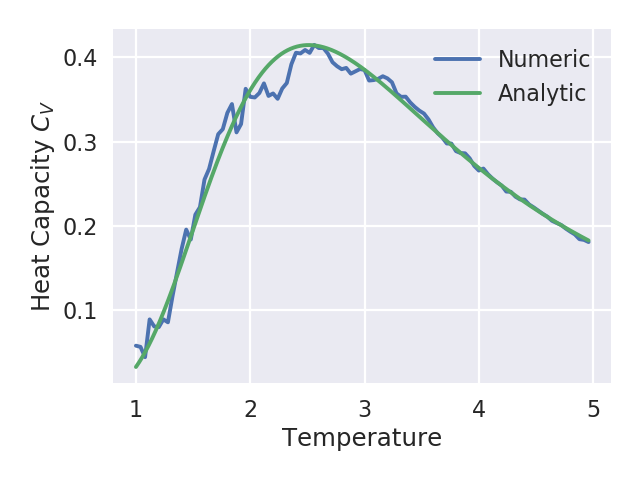
\includegraphics[width=\columnwidth]{figures/L2Ne4.png}
  \caption{$2 \times 2$ lattice with $M = 10^4$ MC iterations.}
  \label{fig:L2Ne4}
\end{figure}
\begin{figure}[H]
  \centering
  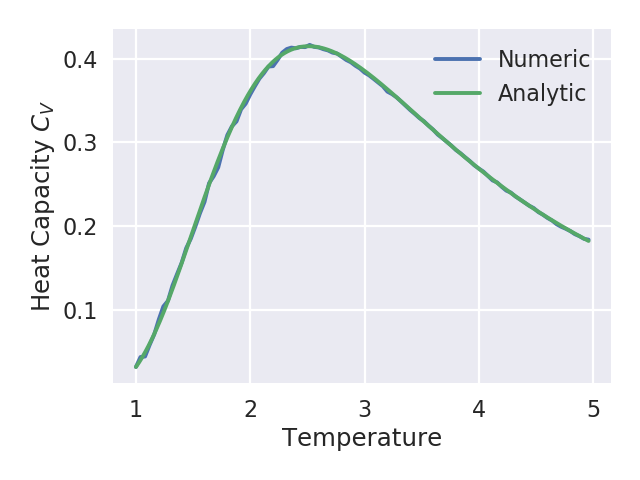
\includegraphics[width=\columnwidth]{figures/L2Ne5.png}
  \caption{$2 \times 2$ lattice with $M = 10^5$ MC iterations.}
  \label{fig:L2Ne5}
\end{figure}
\begin{figure}[H]
  \centering
  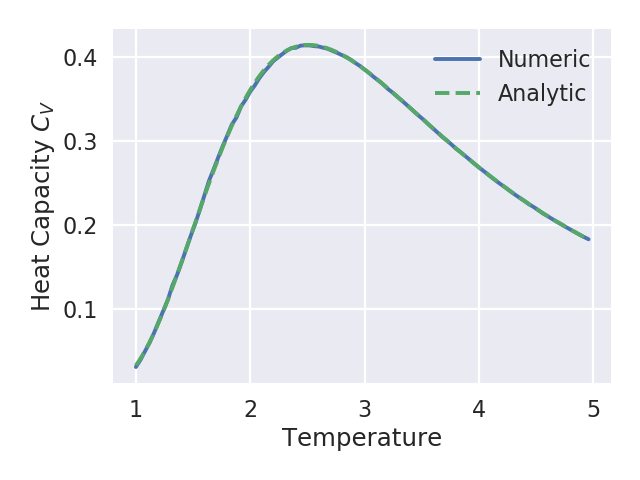
\includegraphics[width=\columnwidth]{figures/L2Ne6.png}
  \caption{$2 \times 2$ lattice with $M = 10^6$ MC iterations.}
  \label{fig:L2Ne6}
\end{figure}

\section{Discussion} \label{sec:discussion}

\section{Conclusion} \label{sec:conclusion}

\bibliography{references}
\blankpage
\appendix
\section{Calculation of analytical expressions for the $2\times2$ lattice.} \label{sec:app}
The mean energy is computed using ~\ref{eq:meanE}.
\begin{align*}
  \mean{E} =
\end{align*}
\blankpage
\end{document}

% Local Variables:
% TeX-engine: luatex
% End:
